\documentclass[11pt]{report}
\usepackage[margin=1in]{geometry}
\usepackage{titlesec}
\usepackage{graphicx}
\usepackage{parskip}
\usepackage{glossaries}
\usepackage{datetime}

\titleformat{\chapter}{\Large\bfseries}{}{0pt}{\huge}
\titlespacing\chapter{0pt}{*1}{*1}
\titlespacing\section{0pt}{*0}{-\parskip}
\titlespacing\subsection{0pt}{*0}{-\parskip}
\titlespacing\paragraph{0pt}{*0}{*3}

\newcommand*{\TitleFont}{
      \usefont{\encodingdefault}{\rmdefault}{b}{n}
      \fontsize{24}{36}
      \selectfont
}
\newcommand{\thickline}{\rule{\textwidth}{1.6pt}}
\newcommand{\thinline}{\rule{\textwidth}{0.4pt}}
\newcommand{\novspace}{\vspace*{-\baselineskip}\vspace*{4pt}}
\renewcommand{\dateseparator}{-}
\let\oldtitle\title
\renewcommand{\title}[1]{\oldtitle{\thickline \\ \novspace \thinline \\ \TitleFont {#1} \thinline \\ \novspace \thickline}}
\newcommand{\tableoffiguresandtables}{\listoffigures\begingroup\let\clearpage\relax\listoftables\endgroup}

\author{
	Evan Milton \\
	Computer and Electronics Engineering \\
	University of Nebraska at Lincoln - Omaha Campus \\
	Electronics Engineering
		\and
	Josh DeWitt \\
	Computer and Electronics Engineering \\
	University of Nebraska at Lincoln - Omaha Campus \\
	Computer Engineering and Mathematics, minor in Computer Science
		\and
	Chad Staley \\
	Computer and Electronics Engineering \\
	University of Nebraska at Lincoln - Omaha Campus \\
	Electronics Engineering
		\and
	James Gehringer \\
	Computer and Electronics Engineering \\
	University of Nebraska at Lincoln - Omaha Campus \\
	Computer Engineering, minor in Computer Science
}
\date{\yyyymmdddate\today}


\titleandsubtitle{CNC Interface \\ Software Requirements Specification}{Submitted in Partial Fulfillment of the Requirements for the B.Sc. Degree, \\ Computer and Electronics Engineering, College of Engineering, \\ University of Nebraska \\ Peter Kiewit Institute, Omaha, Nebraska, U.S.A}

\begin{document}
\maketitle
\tableofcontents
\tableoffiguresandtables
\begin{acronym}
\newacronym{3d}{3-D}{Three-Dimensional}
\newacronym{ceen}{CEEN}{Computer and Electronics Engineering}
\newacronym{ceenc}{\textsc{CeeNC}}{CEEN Numerical Controller}
\newacronym{cnc}{CNC}{Computer Numerical Control}
\newacronym{i2c}{I$^2$C}{Inter-Integrated Circuit}
\newacronym{os}{OS}{Operating System}
\newacronym{pi}{Pi}{Raspberry Pi}
\newacronym{rom}{ROM}{Read-Only Memory}
\newacronym{spi}{SPI}{Serial Peripheral Interface}
\newacronym{srs}{SRS}{Software Requirements Specification}
\newacronym{tcpip}{TCP/IP}{Transmission Control Protocol/Internet Protocol}
\newacronym{ti}{TI}{Texas Instruments}
\newacronym{uart}{UART}{Universal Asynchronous Receiver/Transmitter}
\end{acronym}


\chapter{Introduction}
This section provides an overview of the purpose and scope of the \gls{srs} and introduces the acronyms used within the report.
\section{Purpose}
The purpose of the \gls{srs} is to define the requirements for the software portion of the \gls{ceenc}.
This \gls{srs} was developed in conjuntion with a prototype as part of IEEE Std. 830-1998 section 4.6 \cite[p.~9]{std830}.
This document is intended for anyone that might work on the software at any point in the future.
\section{Scope}
The \gls{ceenc} is a network enabled, configurable \gls{cnc}interface that is compact and affordable.
The \gls{ceenc} accurately and safely drives a set of motors based on G-code files uploaded over the network.
The file will be interpreted in a single board computer and a microcontroller.
 The microcontroller then correctly controls the motors through a motor driver board.
The system can be used to drive a variety of devices, for example a \gls{cnc} Mill or a \gls{3d} printer, through a web interface.
\newline
\newline
The software requirements for this project include a G-code interpreter, ...
\newline
\newline
This subsection should
\newline
a) Identify the software product(s) to be produced by name (e.g., Host DBMS, Report Generator, etc.);
\newline
b) Explain what the software product(s) will, and, if necessary, will not do;
\newline
c) Describe the application of the software being speciÞed, including relevant beneÞts, objectives, and
goals;
\newline
d) Be consistent with similar statements in higher-level specifications (e.g., the system requirements
specification), if they exist.
\section{Definitions, Acronyms, and Abbreviations}
\hspace{12 pt}
\begin{acronym}
\newacronym{3d}{3-D}{Three-Dimensional}
\newacronym{ceen}{CEEN}{Computer and Electronics Engineering}
\newacronym{ceenc}{\textsc{CeeNC}}{CEEN Numerical Controller}
\newacronym{cnc}{CNC}{Computer Numerical Control}
\newacronym{i2c}{I$^2$C}{Inter-Integrated Circuit}
\newacronym{spi}{SPI}{Serial Peripheral Interface}
\newacronym{srs}{SRS}{Software Requirements Specification}
\newacronym{tcpip}{TCP/IP}{Transmission Control Protocol/Internet Protocol}
\newacronym{uart}{UART}{Universal Asynchronous Receiver/Transmitter}
\end{acronym}

\section{References}
%\begin{thebibliography}{9}
%patent

\bibitem{cncpatent}
T. A-Tung, 
”CNC milling machine,” 
U.S. Patent 6,050,760 April 18, 2000

\bibitem{controlmethodpatent}
H. Kawamura, M. Miyata and R. Nozawa, 
”Numerical control method” 
U.S. Patent 4,591,968 May 27, 1986

\bibitem{navpatent}
A. Adamsbaum and J. Deschamps, 
”Navigational process and device for path control,” 
U.S. Patent 3,805,2610 April 16, 1974

\bibitem{executionpatent}
 T. Ichikawa, 
”Numerical control unit with set amount of execution,” 
U.S. Patent 8,036,770 October 11, 2011

\bibitem{webservicepatent}
S.K. Selvaraj and Z. Xiao, 
”Approach For Printing To Web Services-Enabled Printing Devices,” 
U.S. Patent 12/399,884 September 9, 2010

\bibitem{motorcontrolpatent}
S. Ushiyama and K. Matsumoto,  
”Control device of electric motor,” 
U.S. Patent 8,598,818 December 3, 2013

%software-design
\bibitem{piccolo}
	\textit{TMS320F2802x, TMS320F2802xx (Piccolo) MCUs},
	\gls{ti}, Dallas, TX,
	2013, pp. 16.
\bibitem{archlinux}
	\textit{Raspberry Pi | Arch Linux ARM},
	Arch Linux ARM,
	2014, pp. 1.

%economic
\bibitem{3dprintimpact}
	Richard A. D'Aveni,
	\textit{3-D Printing Will Change the World},
	Harvard Business Review, Boston, MA,
	March 2013, pp. 53-54,

\bibitem{3dprintsave}
	Heather Kelly,
	\textit{Study: At-home 3D printing could save consumers thousands},
	CNN Technology Review,
	July 31, 2013

%reliability-analysis
\bibitem{mil217f}
	\textit{Reliability Prediction of Electronic Equipment} (MIL-HDBK-217F), 5th ed.,
	Dept. of Defense, Washington, DC,
	1991, pp. 5-1 - 5-24.
\bibitem{picollo}
	\textit{TMS320F2802x, TMS320F2802xx (Piccolo) MCUs},
	\gls{ti}, Dallas, TX,
	2013, pp. 81, 123.
\bibitem{oki78sr}
	\textit{OKI-78SR Series Fixed Output 1.5 Amp SIP DC/DC Converters},
	Murata Power Solutions, Mansfield, MA,
	2013, pp. 1-3.
\bibitem{lm1117}
	\textit{LM1117-N/LM1171 800mA Low-Dropout Linear Regulator},
	\gls{ti}, Dallas, TX,
	2013, pp. 2, 5.
\bibitem{ieeec951}
	\textit{\gls{ieee} Standard for Safety Levels with Respect to Human Exposure to Radio Frequency Electromagnetic Fields, 3kHz to 300GHz} (\gls{ieee} Std C95.1), 2nd ed.,
	\gls{ieee}, New York, NY,
	2005, pp. 20-25.
\bibitem{ieeenesc}
	\textit{National Electrical Safety Code},
	\gls{ieee}, New York, NY,
	2007, pp 17-20, 32-57.
\bibitem{mil882d}
	\textit{Standard Practice for System Safety} (MIL-STD-882D), 4th ed.,
	Dept. of Defense, Washington, DC,
	2000, pp. 18-20.
\bibitem{emicrystal}
	\textit{EMI-Induced Failures in Crystal Oscillators},
	\gls{ieee} Transactions, vol. 33, no. 4, New York, NY,
	1991, pp. 334-341.

%environmental
\bibitem{3dprintsustain}
	Dr. Philip Reeves,
	\textit{Additive Manufacturing – A supply chain wide response to economic uncertainty and environmental sustainability},
	Econolyst Limited, The Silversmiths, Crown Yard, Wirksworth, Derbyshire, UK
	2013
\bibitem{3dprintenvironment}
	Pearce M. Krieger,
	\textit{"Environmental Life Cycle Analysis of Distributed Three-Dimensional Printing and Conventional Manufacturing of Polymer Products"},
	ACS Sustainable Chemistry \& Engineering: 131002082320002. doi:10.1021,
	2013	

%development analysis
\bibitem{dev_intelligent}
	\textit{Intelligent Stepper Motor Driver with DRV8811/18/24/25},
	\gls{ti}, Dallas, TX,
	2013, pp. 22.
\bibitem{dev_peripherals}
	\textit{Programming TMS320x28xx and 28xxx Peripherals in C/C++},
	\gls{ti}, Dallas, TX,
	2013, pp. 189.
\bibitem{dev_optimize}
	\textit{TMS320C28x Optimizing C/C++ Compiler v6.2.4},
	\gls{ti}, Dallas, TX,
	2013, pp. 24.
\bibitem{dev_drv}
	\textit{DRV8811/18/24/25 Datasheet},
	\gls{ti}, Dallas, TX,
	2013, pp. 22.
\end{thebibliography}

%http://www.cse.chalmers.se/~feldt/courses/reqeng/examples/srs_example_2010_group2.pdf

\section{Overview}
The rest of the \gls{srs} contains sections for the overall description and specific requirements for the software.
The overall description describes how the system will funtion and interact.
It will also describe who the stakeholders are and their roles as well as system constraints and assumptions.
The specific requirements section will explain the requirements of the software in a more detailed manner. 

\chapter{Overall Description}
This section gives a general overview of the factors that affect the product.

\section{Product Perspective}
This section will compare the \gls{ceenc} with other related products and discuss any dependencies.

\subsection{Similar Products}
Before beginning design of the \gls{ceenc}, several alternate \gls{cnc} interfaces were analyzed to understand the current standards and user needs.
While several \gls{cnc} interfaces exist, the \gls{ceenc} has added focus on the usability and lower cost than the alternatives.
\paragraph{MakerBot}
The MakerBot is considered the leader in the current \gls{3d} printer market.
The interface software is MakerBot Desktop, or the older versions were MakerWare.
The MakerBot software allows a user to scan in models and upload files to be printed.
Currently, there is not support for sending files over WiFi, only over USB and Ethernet.
The MakerBot costs around \$2000 depending on the model, although this includes the entire \gls{cnc} machine, not just the driver portion like the \gls{ceenc}.
\paragraph{SmoothieBoard}
SmoothieBoard is an open source driver system with simplistic interfacing software.
It supports Ethernet connections and the system can be accessed through a browser to upload files to the device.
Once a file is uploaded, a command line interface on the device is used to execute files.
The SmoothieBoard costs \$169.97.
\paragraph{EMC2}
EMC2, also known as LinuxCNC, is a freely available \gls{cnc} interface.
It allows for multiple \gls{cnc} configurations, giving flexibility to people who want to build their own \gls{cnc}s.
EMC2 requires a dedicated Linux-based machine and can only operate through a parallel port connector.
\paragraph{OtherMill}
The OtherMill is a new \gls{cnc} controlled by OtherPlan software that costs \$2199.
It allows users to upload a variety of file types, that is converted into G-code interally.
The device offers a command line interface that allows users to send indiviual commands.
The OtherPlan software only supports Mac OS X and the OtherMill must be connected to this computer through USB.

\subsection{Product Dependencies}
The \gls{ceenc} will rely on \gls{tcpip} for communication to a website hosted on the \gls{pi}.
There will be three communication channels in the device, \gls{uart}, \gls{spi}, and gls{i2c}.
The device will be powered from a 12V-36V DC power supply.
The \gls{pi} will be powered from a 5V regulator located on the Control Board.

\section{Product Functions}
The code written for this project is intended to be as modular as possible, avoiding duplication of functionality and increasing testability.
The project relies on free software including the Arch distribution of Linux\cite{archlinux} for the \gls{os} on the \gls{pi}, Apache for web hosting from the \gls{pi}, PHP for creating the back-end services that the website makes calls to, JQuery for creating dynamic web pages, and CuTest, a lightweight unit testing framework for C projects.
As shown in figure~\ref{fig:firmware-hierarchy}, the project contains four software modules: the website control, g-code interpreter, \gls{cnc} driver, and the motor scheduler.
The bootloader on the C2000 is programmed into \gls{rom} and is thus not developed or maintained for this project.
Though not used during normal operation, a set of bash scripts grouped together to create a simple way to set up the \gls{pi} was created to be able to quickly set up the \gls{pi} and get ready for development.

\begin{figure}[!ht]
	\centering
	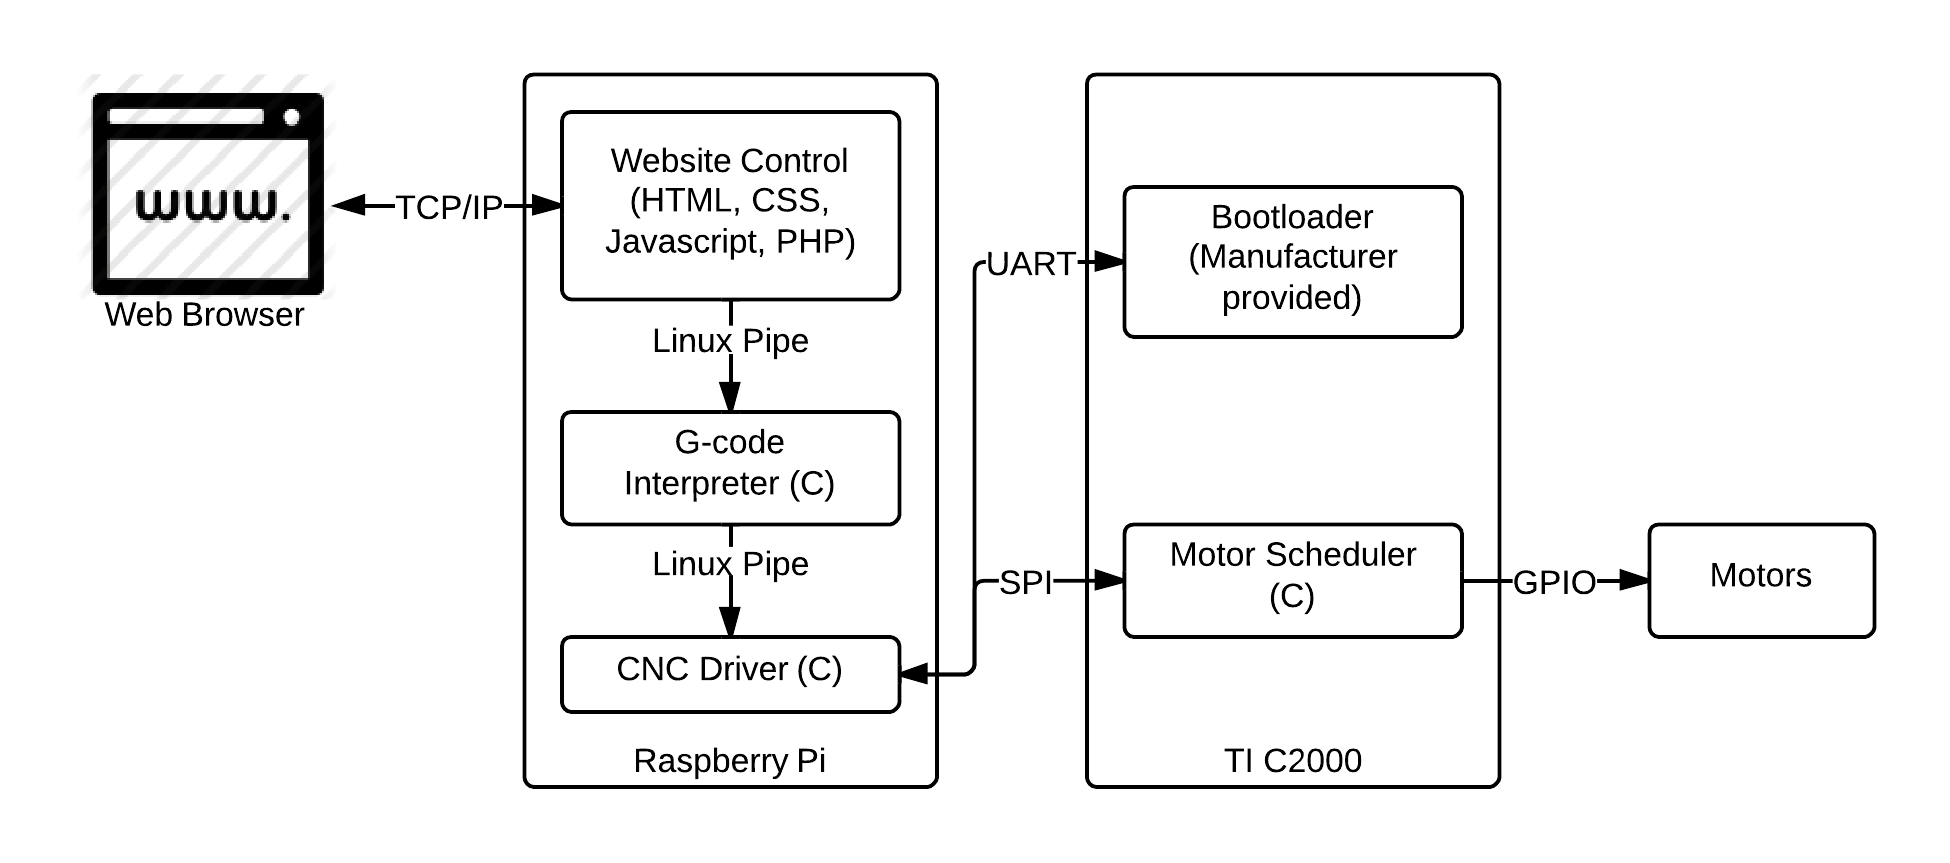
\includegraphics[width=1\textwidth]{firmware-hierarchy.png}
	\caption{Firmware Hierarchy}
	\label{fig:firmware-hierarchy}
\end{figure}

\subsubsection{Website Control}
The website control project is written in HTML, CSS, JavaScript, and PHP and is the main interface between the user and the \gls{cnc}.
The website gives the user the ability to upload, delete, and run g-code files and configure the \gls{cnc}'s characteristics, like gearing ration, maximum speed, and maximum acceleration.

\subsubsection{g-code Interpreter}
The g-code interpreter project is written in C and is responsible for reading g-code line-by-line and interpreting it into instructions for the C2000 to generate the motor pulse trains.
The g-code interpreter listens to a pipe for g-code commands, which may come from a g-code file or directly from the website when the user is homing the machine, then writes to another pipe that is received by the \gls{cnc} driver.
At startup, the g-code interpreter is responsible for driving the state of the C2000, instructing it to home the \gls{cnc}.
The g-code interpreter relies heavily on mathematic formulas created by the software engineer, so many unit tests have been written to ensure proper functionality.

\subsubsection{CNC Driver}
The \gls{cnc} driver project is written in C and is responsible for managing communication channels between the \gls{pi} and C2000 through the \gls{spi} and \gls{uart}.
The g-code interpreter does not write to the \gls{spi} or \gls{uart} directly because these actions require root privileges, so this project was created to allow a single, small program to run as root, while the larger, more frequently changing programs are run by regular users.
The \gls{cnc} driver listens to a pipe for commands to send to the C2000 and forwards them through \gls{spi}, verifying that it is received based on the echo back from the C2000.
The \gls{cnc} driver also looks for a special command that indicates that the next bytes will be \gls{ti} hex data and the program should reset the C2000 and bootload the device with new code.

\subsubsection{Motor Scheduler}
The motor scheduler project is written in C and is responsible for listening for commands from the \gls{pi} and generating the pulse trains to the motors.
The project is based off an algorithm that requires no floating point operations on the C2000 for generating pulses, saving resources and allowing better real-time performance.
The commands are accepted through \gls{spi} and are acknowledged by echoing back the received data, with the command format specified in a C header file shared between the g-code interpreter and this project.

\section{User Characteristics}
The intended users for the \gls{ceenc} will be hobbyists or students interested in computer numerical control for products such as mills or \gls{3d} printers.
The user will be familiar with web interfaces and have access to a \gls{cnc} machine for the interface.
Technical expertise will vary from those who purchase a \gls{cnc} machine pre-assembled to those who make their own and have an understanding of the mechanics involved.
Design of the product will be simple and targeted to those who have little experience with the mechanics involved in a \gls{cnc}.

\section{Constraints}
The major constraints for this project are computational requirements, interface requirements, peripheral requirements, power requirements, packaging requirements, time, and cost.

\subsection{Computational Requirements}
The main computational requirement for this project is the conversion of G-code commands to motor control functions.
The secondary computational requirement is the count and timing of stepper motor steps.
The \gls{pi} will handle software conversion while the microcontroller will handle the timing and count of the motor steps.
When a G-code design file is uploaded and sent to the \gls{pi}, the \gls{pi} will convert the code into commands that can be sent to the microcontroller over a \gls{spi} bus.
This conversion may occur in non-real-time.
The microcontroller will handle the timing and counting of the motor control functions.
Once the microcontroller receives the motor control commands, it will output appropriate step and direction data to the motor drivers.
The motor control data must execute in real-time to ensure accuracy.
The microcontroller must be capable of outputting a step frequency of at least 10kHz and within 5\% of the target frequency for any frequency in that range.
The microcontroller will also monitor the status of the motor drivers and communicate any faults back to the computer.

\subsection{Interface Requirements}
The microcontroller must have at least 8 outputs for stepper motor control, 4 inputs for stepper motor home, 1 input for the motor driver faults, 1 input for an emergency stop, and 1 PWM output for DC motor control.
Between the computer and microcontroller, an additional 16 outputs must be available for use by the end user as part of the project success criteria.
The additional outputs may be accomplished by using serial to parallel shift registers or an \gls{i2c} port expander.
If shift registers are used, 3 output pins will be required by either the pi or microcontroller for the clock, storage input, and data input.
If an \gls{i2c} port expnader is used, 2 output pins will be required by either the \gls{pi} or the microcontroller for the \gls{i2c} channel.
All digital logic will be 3.3V.
To protect the \gls{pi} and microcontroller, opto-isolators will be used at the input and output of the motor drivers.

\subsection{Peripheral Requirements}
The \gls{pi} will require either Ethernet or Wi-Fi capabilities to connect to a website.
The \gls{pi} must have a one channel \gls{spi} bus to communicate with the microcontroller. 
The microcontroller must have a one channel \gls{spi} bus to communicate with the \gls{pi}.
The microcontroller must have a JTAG port for programming.
The microcontroller may require up to four 16-bit timers for motor step counting.

\subsection{Power Constraints}
The system will accept one DC power supply that can be between 14V and 36V.
The system will draw no more than 10A including the current required for the motors.
A 5V power regulator will be used to supply the computer.
A 3.3V power regulator will be used to supply the microcontroller and ICs.
The 14-36V DC rail will be used to supply the motor drivers. 

\subsection{Packaging Constraints}
The finished project must be professionally packaged.
The footprint of the packaging will likely not be much larger than the footprint of largest PCB which is expected to be approximately 87mm x 56 mm, however this is not a requirement.
The size of the finished project will not impact performance in a considerable manner.

\subsection{Time and Cost Constraints}
Current CNC interfaces require use of a full computer system in combination with a motor driver platform.
These setups can cost upwards of \$500.
This project will combine and simplify these hardware and software requirements for a cost of under \$100.
Since this is a student project, there is 

\section{Assumptions and Dependencies}
This subsection of the SRS should list each of the factors that affect the requirements stated in the SRS.
These factors are not design constraints on the software but are, rather, any changes to them that can affect
the requirements in the SRS. For example, an assumption may be that a speciÞc operating system will be
available on the hardware designated for the software product. If, in fact, the operating system is not available,
the SRS would then have to change accordingly.
\chapter{Specific Requirements}
This section of the SRS should contain all of the software requirements to a level of detail sufÞcient to enable designers to design a system to satisfy those requirements, and testers to test that the system satisÞes those requirements. 
Throughout this section, every stated requirement should be externally perceivable by users, operators, or other external systems.
These requirements should include at a minimum a description of every input (stimulus) into the system, every output (response) from the system, and all functions performed by the system in response to an input or in support of an output.
As this is often the largest and most important part of the SRS,


\end{document}